\newpage

\begin{landscape}

\section{Projektstrukturplan}\label{sec:Projektstrukturplan}
In Projektstrukturplan sind die verschiedenen Meilensteine und die genaue Einteilung der Personenstunden im Verlauf des Semesters ersichtlich.

\subsection{Arbeitspakete und Zeitplan}\label{subsec:Arbeitspakete_und_Zeitplan}

\begin{figure}[h]
   \centering
   \noindent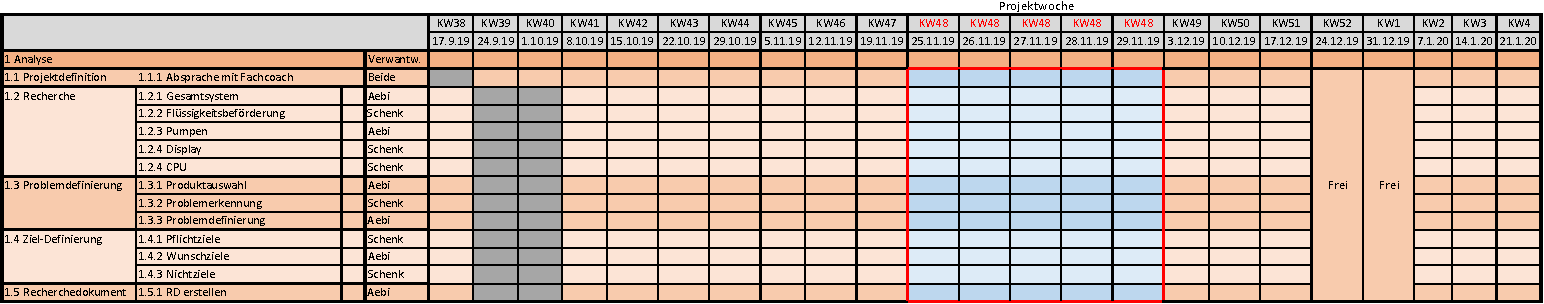
\includegraphics[width=\linewidth,keepaspectratio]{graphics/Analyse.pdf}
%   \caption[Beispielbild]{Beispielbild}
   \label{pic:Analyse}
\end{figure}

\begin{figure}[h]
   \centering
   \noindent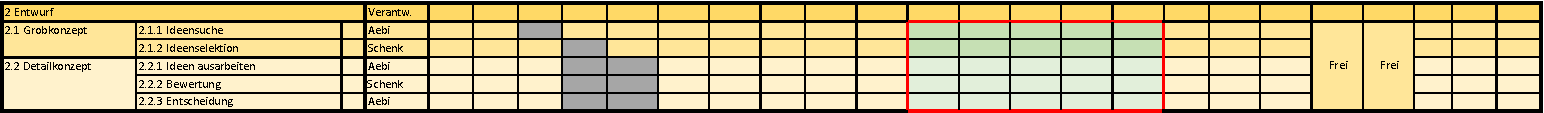
\includegraphics[width=\linewidth,keepaspectratio]{graphics/Entwurf.pdf}
%   \caption[Beispielbild]{Beispielbild}
   \label{pic:Entwurf}
\end{figure}

\begin{figure}[h]
   \centering
   \noindent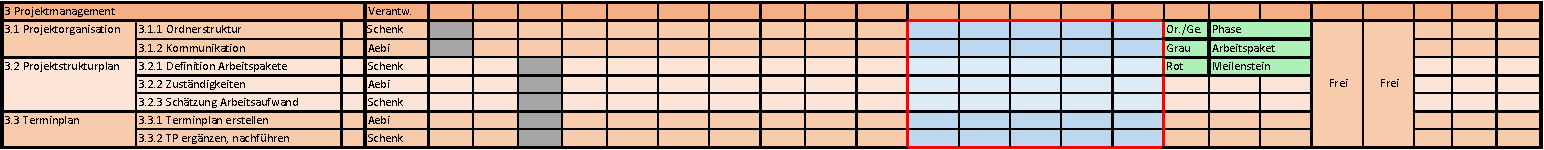
\includegraphics[width=\linewidth,height=.9\textheight,keepaspectratio]{graphics/Projektmanagemant.pdf}
%   \caption[Beispielbild]{Beispielbild}
   \label{pic:Projektmanagement}
\end{figure}
\vfill
\clearpage
\begin{figure}[h]
   \centering
   \noindent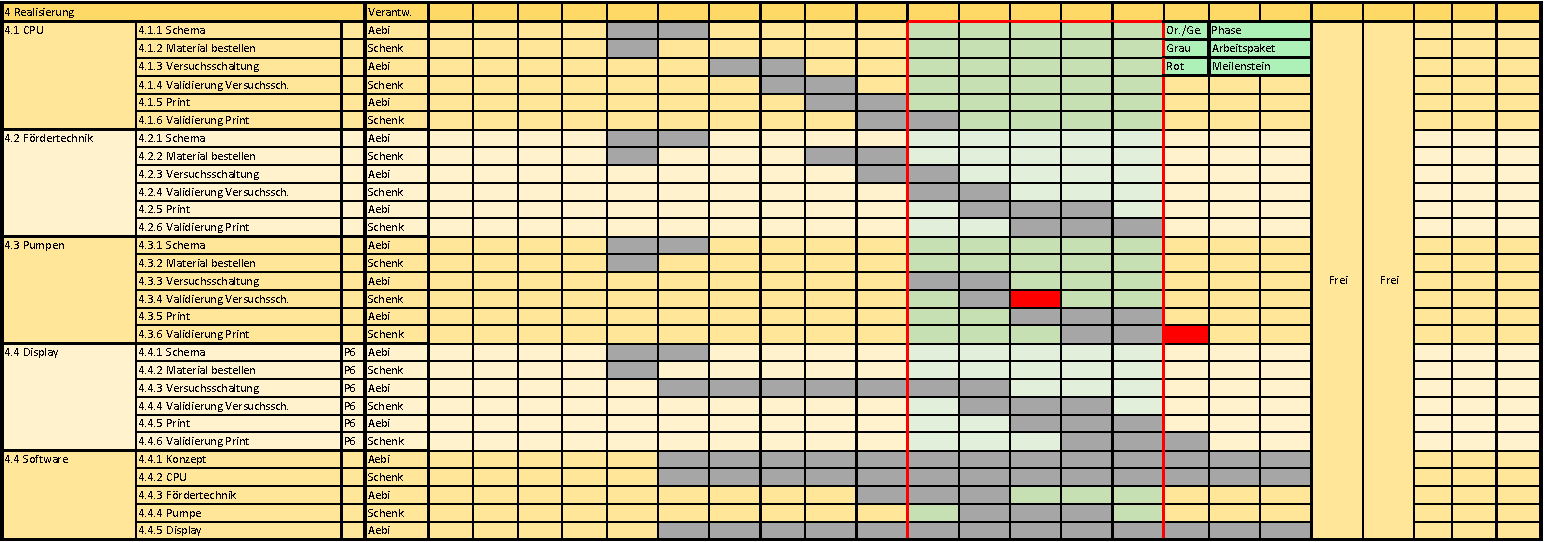
\includegraphics[width=\linewidth,keepaspectratio]{graphics/Realisierung.pdf}
%   \caption[Beispielbild]{Beispielbild}
   \label{pic:Realisierung}
\end{figure}
\clearpage
\subsection{Meilensteine}\label{subsec:Meilensteine}
 \begin{figure}[h]
   \centering
   \noindent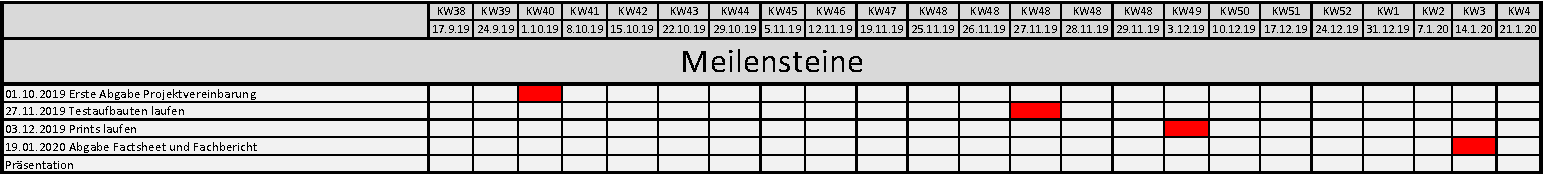
\includegraphics[width=\linewidth,height=.9\textheight,keepaspectratio]{graphics/Meilensteine.pdf}
%   \caption[Beispielbild]{Beispielbild}
   \label{pic:Meilensteine}
\end{figure}
\vfill
\end{landscape}